\chapter{Related Work} %todo: citations, images
\label{State of the art}

In this chapter, we introduce the main ideas and methods that will form the foundation for our approach and evaluation in Chapter 3.
First, we will capture the fundamental concepts of Deep Learning in an image segmentation context. Regarding this, we will introduce Multilayer Perceptrons (MLPs) and Convolutional Neural Networks (CNNs) alongside the basic concepts of optimization theory. Afterwards, we will go over the way the so called Transformer Networks use attention mechanisms, to create a new way of feature representation of sequenced input data. This Transformer Network architecture is then extended to handle image data. Some extensions are then introduced, that are adopted in @todo


\section{Convolutional Neural Networks (CNNs)}

Convolutional neural networks (CNNs) are a class of deep learning models designed to learn features directly from data, making them especially effective for inputs with spatial structure \cite{LeCun.1989}. Rather than relying on handcrafted descriptors, CNNs acquire representations through convolutional layers, where small filters slide across the input to detect local patterns. Early layers typically respond to simple structures such as edges or gradients, while deeper layers combine these responses into progressively more abstract features, including textures, shapes, or semantic concepts.

To expand their representational power, convolutional operations are followed by non-linear activation functions, most commonly the rectified linear unit (ReLU). These non-linearities prevent the network from collapsing into a purely linear model and allow it to approximate complex functions. Pooling layers are often included to reduce the spatial resolution of feature maps by summarizing local neighborhoods. This downsampling lowers computational cost, introduces translational invariance, and emphasizes the most salient information. Together, convolutions, non-linearities, and pooling operations form a hierarchy that transforms raw data into increasingly abstract and task-relevant features.

Additional design choices such as batch normalization, dropout, and skip connections further improve stability, regularization, and information flow. Nonetheless, the core strength of CNNs lies in their hierarchical feature acquisition, which enables robust generalization and has established them as a fundamental architecture in modern machine learning across diverse domains.

\subsection{ImageNet}

The development of modern deep learning for image analysis is closely linked to the ImageNet Large Scale Visual Recognition Challenge (ILSVRC). Introduced in 2009, ImageNet is a large-scale, annotated image database containing over 14 million images across thousands of object categories. The ILSVRC provided a benchmark for evaluating classification and detection methods on a massive and diverse dataset, driving rapid advancements in computer vision. 

\begin{figure}
    \centering
    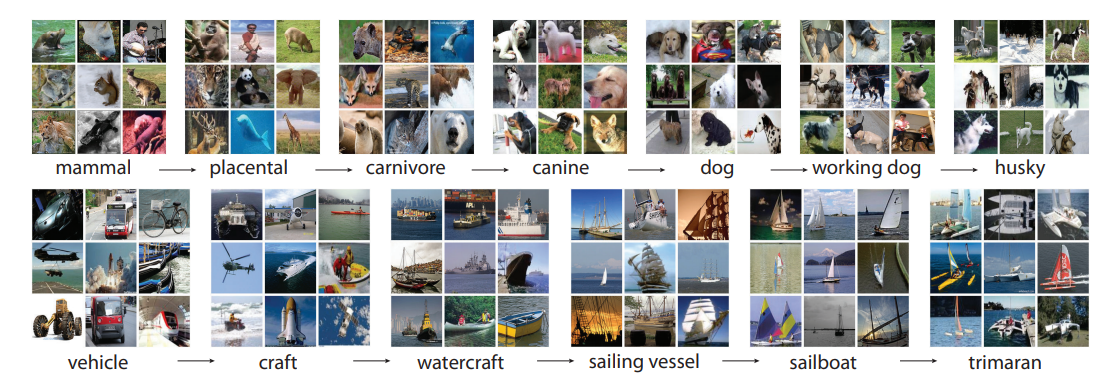
\includegraphics[width=1\linewidth]{Images/SOTA/ImageNet.png}
    \caption{Example Images from the ImageNet dataset.}
    \label{fig:ImageNet}
\end{figure}

A major breakthrough came in 2012 with AlexNet, a deep convolutional neural network (CNN) that significantly outperformed previous approaches on the ImageNet classification task. This success demonstrated the power of deep architectures trained on large datasets and marked the beginning of widespread adoption of CNNs for a variety of vision tasks. Following AlexNet, CNNs evolved through multiple directions to improve performance. Increasing network depth and width allowed models to capture more complex patterns and richer feature hierarchies. Enhanced connectivity patterns, such as skip connections and residual blocks, improved gradient flow and facilitated training of very deep networks. In addition, more sophisticated forms of convolution, including dilated and grouped convolutions, allowed for multi-scale feature extraction and more efficient parameter usage.

These architectural advances enabled CNNs to become the backbone for a wide range of vision applications, from image classification and object detection to segmentation and beyond. The combination of hierarchical feature extraction, non-linear activations, and spatial aggregation operations continues to make CNNs highly effective and generalizable across diverse domains, including medical and biological imaging, where large annotated datasets are often limited. 
While the developement of CNNs has benefitted a lot from the ImageNet dataset, also novel architectures such as Transformer based models, which be later introduced, make use of the diverse ImageNet dataset to be pretrained for many downstream tasks. 

% \subsection{Convolution Operation}
% In a 2D convolution operation, a small matrix called a \emph{kernel} or \emph{filter} (denoted $\mathbf W$) is slid across an input matrix $\mathbf X$. At each position, the element-wise products of the overlapping values between the kernel and the corresponding region of the input are summed to produce a single value in the output matrix $\mathbf Y$. This process is repeated as the kernel moves over all possible positions in the input matrix, typically with a stride of 1 and with or without padding.

% Formally, for a kernel of size $k \times k$, an input matrix of size $m \times n$, and an output matrix of size $(m-k+1) \times (n-k+1)$ (assuming 'valid' padding), the convolution operation at position $(i,j)$ is defined as:
% \begin{equation}
% Y_{i,j} = \sum_{u=0}^{k-1} \sum_{v=0}^{k-1} X_{i+u,\, j+v} \cdot W_{u,v}.
% \end{equation}

% As an example, given the input matrix \({\mathbf{X}}\) and kernel \({\mathbf{X}}\):
% \[
% \mathbf{X} = 
% \begin{bmatrix}
% 1 & 2 & 3 & 0 \\
% 0 & 1 & 2 & 1 \\
% 3 & 0 & 1 & 2 \\
% 2 & 1 & 0 & 1 \\
% \end{bmatrix}
% \quad
% \mathbf{W} = 
% \begin{bmatrix}
% 1 & 0 \\
% 0 & 1 \\
% \end{bmatrix},
% \]
% the output value at position $(1,1)$ is computed as
% \[
% Y_{1,1} = (1 \times 1) + (2 \times 0) + (0 \times 0) + (1 \times 1) = 2 .
% \]
% This computation is then repeated for every valid position where the kernel fully overlaps the input, resulting in the output matrix.

% In practice, convolution operations can also be configured with additional parameters such as \textit{padding} and \textit{stride}. Padding adds extra rows and columns (typically filled with zeros) around the border of the input matrix, allowing the kernel to cover edge regions and control the spatial size of the output. The stride defines the step size with which the kernel moves across the input. Increasing the stride reduces the spatial dimensions of the output feature map, effectively downsampling the input while still capturing local patterns. These options provide flexibility in designing convolutional layers for various use cases, such as reducing spatial resolution or preserving the input size.

% In practical applications, multiple kernels are typically applied in parallel to detect different patterns or features in the input, resulting in multiple output feature maps.

% \begin{figure}[!ht]
% \centering
% \begin{tikzpicture}[
%     2d-arr/.style={matrix of nodes, row sep=-\pgflinewidth, column sep=-\pgflinewidth, nodes={draw}}
%   ]

%   \matrix (mtr) [2d-arr] {
%   0 & 1 & 1 & |[fill=red!30]| 1 & |[fill=red!30]| 0 & |[fill=red!30]| 0 & 0\\
%   0 & 0 & 1 & |[fill=red!30]| 1 & |[fill=red!30]| 1 & |[fill=red!30]| 0 & 0\\
%   0 & 0 & 0 & |[fill=red!30]| 1 & |[fill=red!30]| 1 & |[fill=red!30]| 1 & 0\\
%   0 & 0 & 0 & 1 & 1 & 0 & 0\\
%   0 & 0 & 1 & 1 & 0 & 0 & 0\\
%   0 & 1 & 1 & 0 & 0 & 0 & 0\\
%   1 & 1 & 0 & 0 & 0 & 0 & 0\\
%   };

%   \node[below=of mtr-5-4] {$\mathbf I$};

%   \node[right=0.2em of mtr] (str) {$*$};

%   \matrix (K) [2d-arr, right=0.2em of str, nodes={draw, fill=teal!30}] {
%     1 & 0 & 1 \\
%     0 & 1 & 0 \\
%     1 & 0 & 1 \\
%   };
%   \node[below=of K-3-2] {$\mathbf K$};

%   \node[right=0.2em of K] (eq) {$=$};

%   \matrix (ret) [2d-arr, right=0.2em of eq] {
%   1 & 4 & 3 & |[fill=blue!80!black!30]| 4 & 1\\
%   1 & 2 & 4 & 3 & 3\\
%   1 & 2 & 3 & 4 & 1\\
%   1 & 3 & 3 & 1 & 1\\
%   3 & 3 & 1 & 1 & 0\\
%   };
%   \node[below=of ret-4-3] {$\mathbf{I * K}$};

%   \draw[dashed, teal] (mtr-1-6.north east) -- (K-1-1.north west);
%   \draw[dashed, teal] (mtr-3-6.south east) -- (K-3-1.south west);

%   \draw[dashed, blue!80!black] (K-1-3.north east) -- (ret-1-4.north west);
%   \draw[dashed, blue!80!black] (K-3-3.south east) -- (ret-1-4.south west);

%   \foreach \i in {1,2,3} {
%       \foreach \j in {4,5,6} {
%           \node[font=\tiny, scale=0.6, shift={(-1.2ex,-2ex)}] at (mtr-\i-\j) {$\times \pgfmathparse{int(mod(\i+\j,2))}\pgfmathresult$};
%         }
%     }

% \end{tikzpicture}
% \caption{Illustration of a 2D convolution operation: a $3 \times 3$ kernel $\mathbf W$ slides over a $4 \times 4$ input matrix $\mathbf X$. At each position, the element-wise products of the overlapping elements are summed to produce one value in the result matrix $\mathbf Y$. Highlighted are the current overlapping elements in $\mathbf X$ and the corresponding value in $\mathbf Y$.}
% \label{fig:2d_convolution_horizontal}
% \end{figure}


% The role of these convolutional layers is to perform hierarchical feature extraction. Early layers tend to learn simple and general features, while deeper layers combine these into more abstract representations. To reduce computational complexity and improve generalization, CNNs often include pooling layers, such as max pooling, which downsample the feature maps by retaining only the most prominent values in a neighborhood. This reduces the dimensionality of the data and merges semantically similar features, complementing the convolutional layer whose primary role is to detect local feature combinations from the previous layer \cite{LBH15}.


\subsection{U-Net Architecture}

A widely adopted convolutional neural network architecture for biomedical image segmentation is the \textit{U-Net}, introduced by Ronneberger et al. in 2015. The U-Net was specifically designed for tasks where precise localization is essential, such as cell segmentation in microscopy images. Its name derives from its characteristic U-shaped architecture, consisting of a contracting path (encoder) and an expansive path (decoder).

\begin{figure}[!ht]
    \centering
    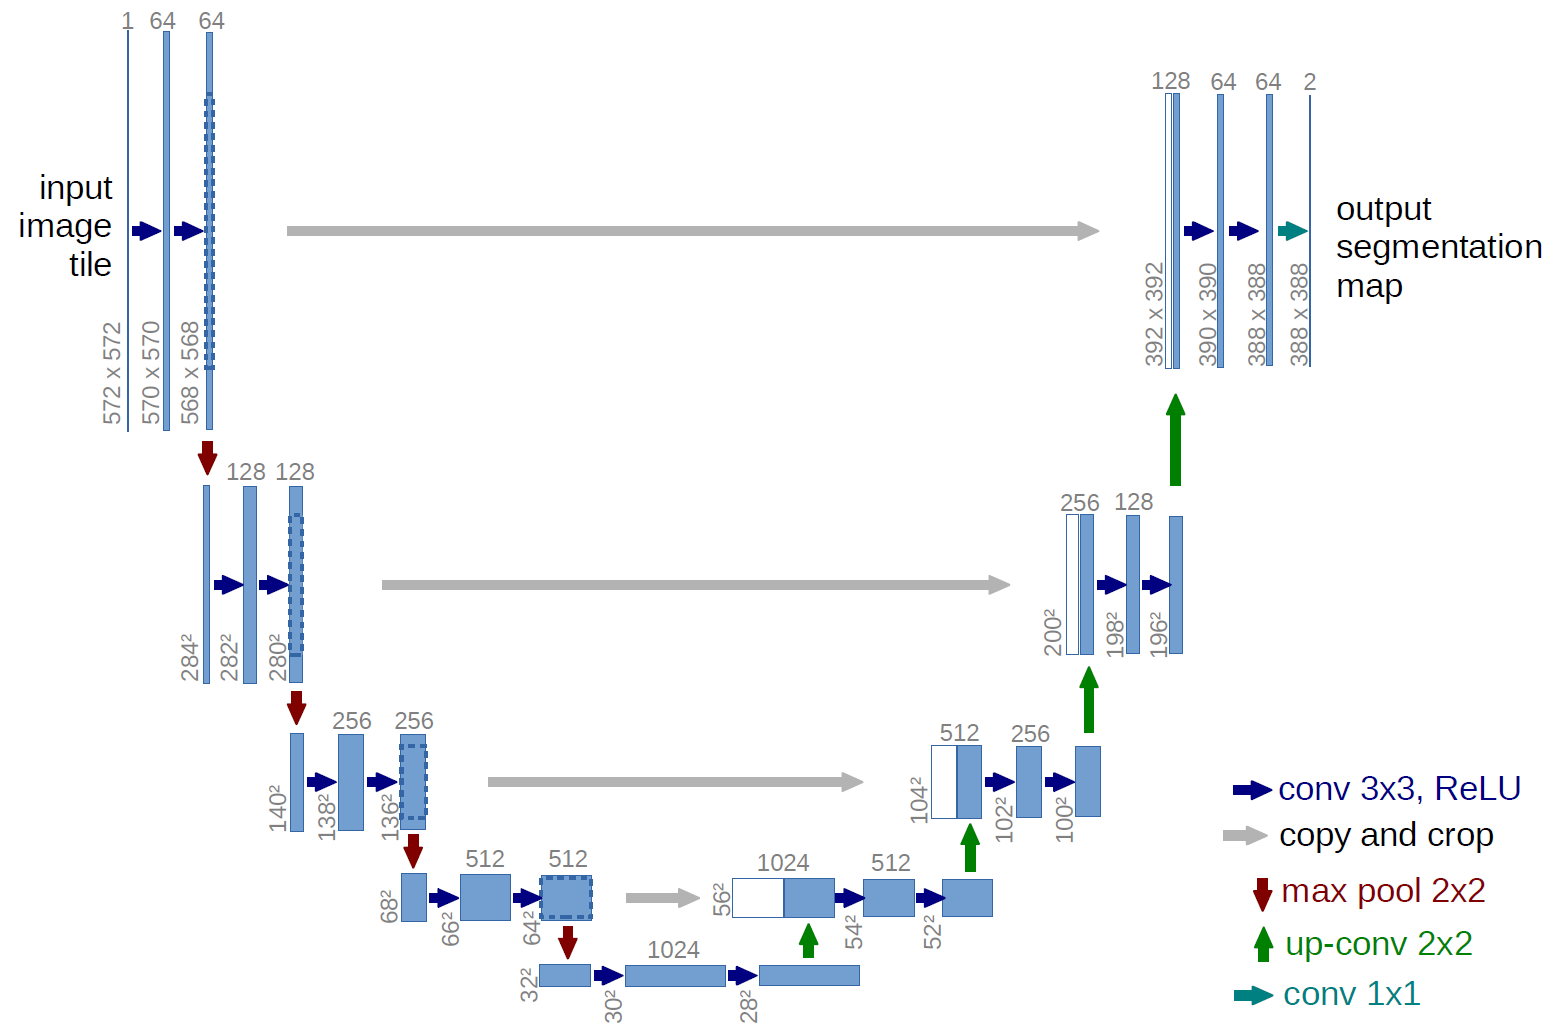
\includegraphics[width=0.8\textwidth]{Images/SOTA/u-net-architecture.png}
    \caption{Schematic illustration of the U-Net architecture for image segmentation. The network consists of a contracting path (left side) to capture context via successive convolutional (3×3, ReLU) and max pooling (2×2) operations, and an expansive path (right side) that enables precise localization through up-convolutions (2×2) and concatenation with high-resolution features from the contracting path. The final segmentation map is generated using a 1×1 convolution. Feature map sizes and channel numbers are indicated for each layer.}
    \label{fig:unet}
\end{figure}


The \textbf{contracting path} progressively reduces the spatial dimensions of the input while increasing the number of feature channels. This is achieved through repeated applications of convolutional layers followed by non-linear activations and downsampling operations such as max pooling. The purpose of this path is to capture the contextual and semantic information of the input image at various scales.

The \textbf{expansive path}, on the other hand, restores the spatial resolution through a sequence of upsampling operations (e.g., transposed convolutions) and concatenations with corresponding feature maps from the contracting path via \textit{skip connections}. These skip connections provide fine-grained spatial details from earlier layers, improving the precision of the segmentation boundaries.

Formally, the segmentation prediction can be seen as a pixel-wise classification problem, where the final layer of the U-Net outputs a probability map indicating the likelihood of each pixel belonging to a particular class (e.g., foreground or background in binary cell segmentation). The combination of hierarchical feature extraction and precise localization makes the U-Net particularly effective for segmenting structures of varying size and shape, as commonly encountered in biomedical images.

U-Net and its derivatives have since become the backbone of many state-of-the-art cell segmentation pipelines in both fluorescence and label-free imaging modalities.

\section{Image Segmentation}

In this section, we will introduce the main types of segmentation in image data and will further explain the techniques that help us achieve an accurate segmentation result. We will learn how modified learning objectives will lead to better results and 


\subsection{Semantic and Instance Segmentation}


The vanilla U-Net assigns pixels to distinct, predifined classes. Usually, at the last layer of the decoder path, the original image resolution is restored (neglecting the missing pixels from unpadded convolutions). At this point, one would map the channel feature map depth (e.g. 64 for vanilla U-Net) via a 1x1 convolution to the amount of classes each pixel can be assigned to. Thereby one ends up having a probability distribution of predefined classes over all pixels. Logits are mapped to probabilities with Soft-Max and with Non-Maximum-Supression (NMS), each pixel is assigned to a class, so in the end the resolution corresponds to $\mathbf{H \times W}$ with each pixel integer value corresponding to a certain class. These classes can represent all kinds of types, such as binarary values like foreground/background (cell or no cell), or for modern use cases, surrounding objects on a street. This type of segmentation is refered to as \textit{semantic segmentation}. Oftentimes some other sophisticated post processing methods like binary closing or removal objects with size below a certain threshold are applied.

\begin{figure}[!ht]
    \centering
    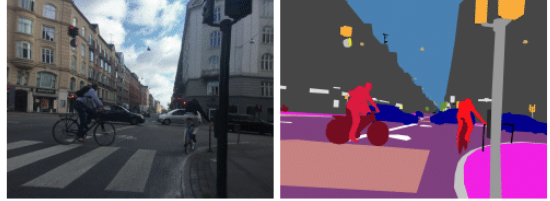
\includegraphics[width=0.6\textwidth]{Images/SOTA/SemanticSeg.png}
    \caption{Semantic Segmentation in the Traffic Environment using the DeepLabv3+ Model}
    \label{fig:semanticSeg}
\end{figure}


For many applications, it is desirable to use a framework that not only separates image regions into semantic classes, but also assigns each object instance within the same class a unique identifier. This task is known as instance segmentation.

A common strategy is to first perform semantic segmentation and then separate individual instances in a post-processing step (a bottom-up approach). However, such methods are often prone to errors, for example when adjacent objects of the same class touch or overlap, leading to under-segmentation (merging of multiple cells) or over-segmentation (splitting a single cell into several fragments).

Alternatively, instance segmentation can be formulated as detecting object proposals via bounding boxes, which are then refined into masks, as done in methods like Mask R-CNN. While effective in many domains, this top-down approach becomes inaccurate in dense cellular images where bounding boxes frequently overlap, making NMS unreliable.

For cellular instance segmentation, it is therefore common to edit the learning objective itself so that the model directly predicts instance-specific features (e.g., object centers, flow fields, or boundary cues). These features can then be leveraged during post-processing to produce accurate boundaries and clearly separated instances. StarDist for example, directly predicts a set of ray distances to the object boundary for every pixel. Fusing this feature with a per pixel cell probability map, the set of proposed polygon shaped objects can be accurately post processed with NMS to predict even spatially dense distributed cells.

\begin{figure}[!ht]
    \centering
    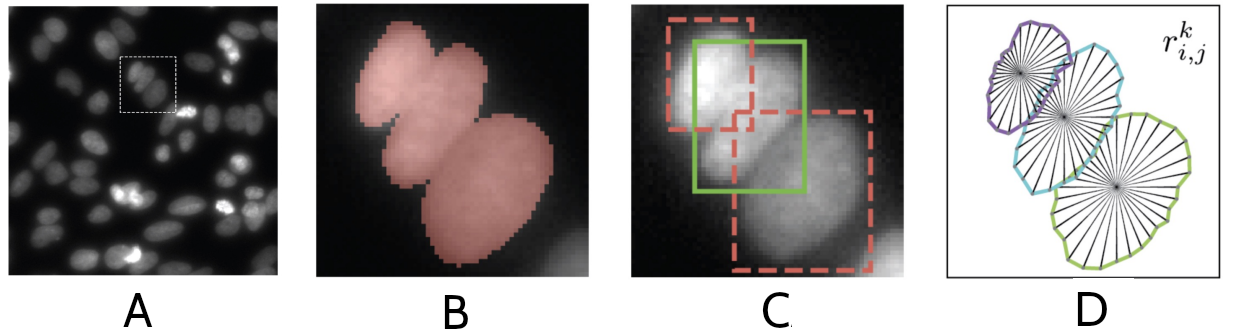
\includegraphics[width=0.9\textwidth]{Images/SOTA/stardist.png}
    \caption{Different instance segmentation methods, A: original image, B: Bottom-up approach, C: Top-down approach, D: Direct instance segmentation, where the model predicts instance-specific features that are used to delineate individual objects.}
    \label{fig:StarDist}
\end{figure}

\subsection{Cellpose}

While StarDist aims to predict distance maps to the object boundary, Cellpose introduced a novel approach by predicting spatial gradients that point toward the center of each cell. Classical approaches such as the watershed algorithm rely on intensity basins in the image to define object regions, but in many microscopy images, cells exhibit multiple intensity basins due to inhomogeneous labeling or nuclear exclusion of fluorescent markers. To overcome this limitation, Cellpose constructs an intermediate representation of each cell as a single smooth topological basin.

\begin{figure}[!ht]
    \centering
    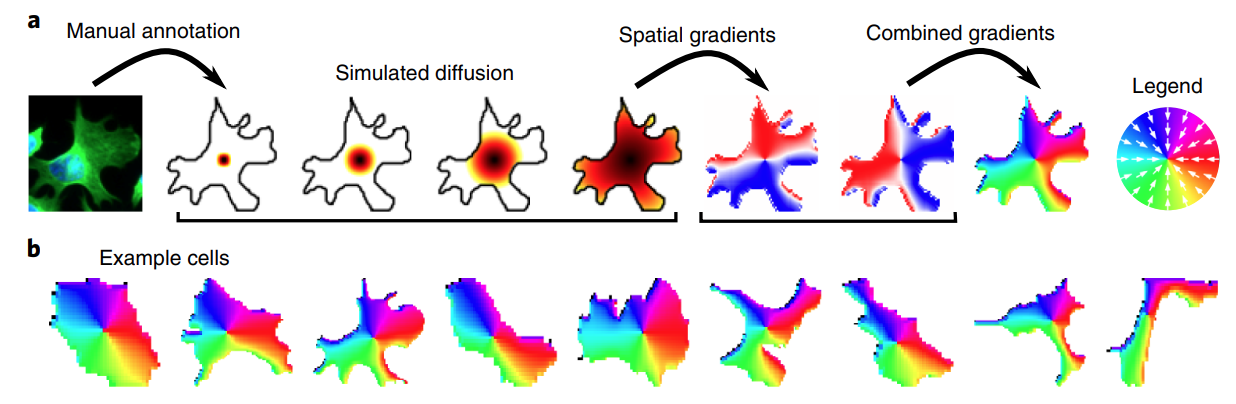
\includegraphics[width=0.9\textwidth]{Images/SOTA/cellpose_learning_objective.png}
    \caption{t-SNE embeddings of image styles from cellpose pretraining data.}
    \label{fig:cellpose_learning_objective}
\end{figure}

These topological maps are generated from manually annotated masks using a simulated diffusion process, which produces horizontal and vertical gradients pointing toward the center of each cell. The network is then trained to predict 3 channels: 2 channels for xy gradients together with a channel per pixel cell probability. At post processing, the predicted gradients define a vector field through which pixels are iteratively routed toward their corresponding cell centers. By grouping pixels that converge to the same point, the network recovers individual cell instances with accurate shapes, which are further refined using the predicted binary mask to remove pixels outside of cells.

Similarly to StarDist, the first launch of cellpose transforms manually annotated masks to the learning objective shape and uses a U-Net which maps the features to the learning objective channels with conv2d layers. Global average pooling of the lowest-resolution features is used to extract an image 'style' vector, which is incorporated throughout the upsampling stages to account for differences in imaging modalities and staining patterns. Insterestingly, plotting the style vectors with t-SNE shows clear distinctions in cell modalities, as k-means clustering groups similar cell types together.

\begin{figure}[!ht]
    \centering
    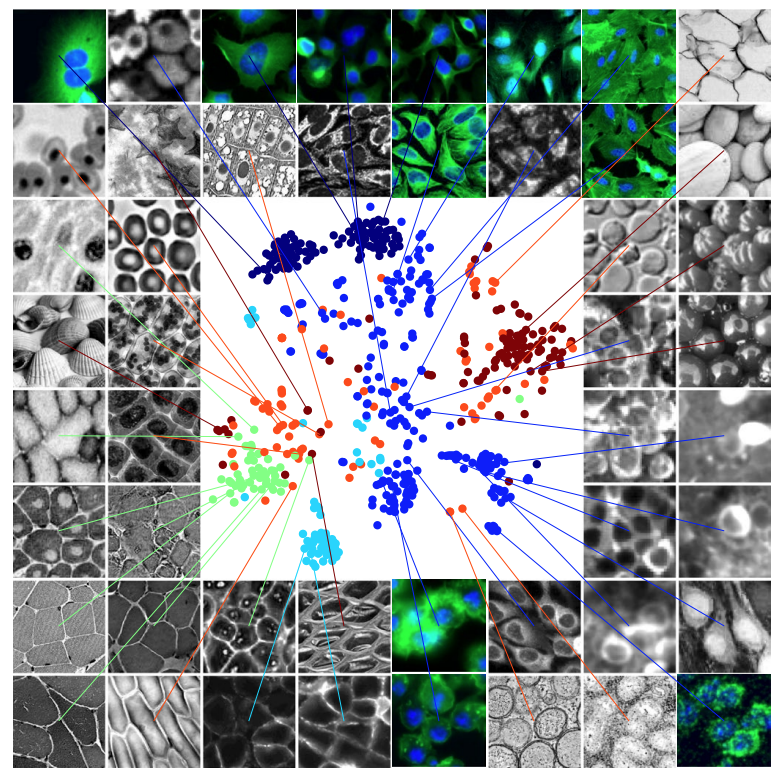
\includegraphics[width=0.6\textwidth]{Images/SOTA/tSNE_cellpose.png}
    \caption{t-SNE embedding of image styles from cellpose pretraining data.}
    \label{fig:t-SNE}
\end{figure}


In practice, it turns out that this feature representation performs best across many benchmarks and is considered state-of-the-art for cell segmentation. Although for specialized datasets, StarDist performs very similarly well, Cellpose's learning objective generalizes better across diverse cell types and imaging modalities. The model itself is considered a foundation model for cell segmentation, due to its very heavy pretraining. Therefore, it performs very well on unseen data, even without any finetuning. 


\subsection{Loss Functions and Metrics}

The loss function, denoted by $\mathcal{L}$, plays a central role in training neural networks by providing a quantitative measure of the error between the predicted output and the true target values. During training, the network's parameters are updated to minimize this loss, improving its predictive performance on the given task.

While loss functions guide the optimization process during training, \textit{evaluation metrics} serve to assess the quality of the model's predictions, typically on a separate validation or test set. Metrics quantify different aspects of performance that are relevant to the problem at hand and are especially important in applications such as cell segmentation, where a model's utility is not solely determined by its training loss.

In cell segmentation tasks, common evaluation metrics include the \textit{Intersection over Union (IoU)}, \textit{Dice coefficient}, and \textit{Average Precision (AP)}, all of which compare the predicted segmentation masks to the ground truth annotations.

The \textbf{Intersection over Union (IoU)}, also known as the Jaccard index, measures the overlap between the predicted mask $P$ and the ground truth mask $G$ relative to their union:
\[
\mathrm{IoU}(P, G) = \frac{|P \cap G|}{|P \cup G|}
\]
A higher IoU indicates a better agreement between prediction and ground truth, with a value of 1 representing perfect overlap.

The \textbf{Dice coefficient}, closely related to IoU, is another overlap-based metric commonly used in segmentation tasks. It is defined as:
\[
\mathrm{Dice}(P, G) = \frac{2 |P \cap G|}{|P| + |G|}
\]
Like IoU, the Dice coefficient ranges from 0 to 1, where a value of 1 indicates perfect correspondence between the predicted and ground truth masks. Compared to IoU, the Dice score tends to be slightly more forgiving in cases of small object segmentation.

Another widely used metric in instance segmentation is the \textbf{Average Precision (AP)}. It summarizes the precision-recall curve into a single value by integrating over different confidence thresholds. Given precision $\mathrm{Prec}(t)$ and recall $\mathrm{Rec}(t)$ at threshold $t$, the Average Precision is computed as:
\[
\mathrm{AP} = \int_0^1 \mathrm{Prec}(\mathrm{Rec}) \, d\mathrm{Rec}
\]
In practice, this integral is often approximated using discrete recall points. In cell segmentation benchmarks, AP is typically reported at different IoU thresholds (e.g., AP@0.5, AP@0.75) to capture performance at varying levels of prediction-stringency.

Together, the choice of loss function for optimization and the metrics for evaluation provide complementary perspectives: the former drives model improvement during training, while the latter ensures the resulting model performs reliably and meaningfully on the specific segmentation task.


% \subsection{Dropout}

% Dropout, introduced by Srivastava et al. in 2014, is a simple yet effective regularization technique designed to reduce overfitting in neural networks. The core idea is to randomly deactivate a subset of neurons along with their connections during each training iteration. This prevents neurons from becoming overly reliant on specific other units, thereby reducing complex co-adaptations within the network. During training, dropout effectively samples from a large number of different “thinned” networks by randomly omitting different sets of units. At inference time, the full network is used, but with appropriately scaled weights to approximate the average of the many subnetworks seen during training. This technique has been shown to significantly improve generalization performance and often outperforms other regularization methods \cite{SHK+14}.

% One major advantage of dropout is its low computational cost, especially relative to its performance gains. Additionally, dropout integrates seamlessly with a wide variety of model architectures and training procedures. It is particularly effective for models using distributed representations and can be easily combined with stochastic gradient descent \cite{GBC16}.


% \subsection{Batch Normalization}

% % Batch normalization, introduced by Ioffe and Szegedy in 2015, addresses the problem of internal covariate shift by normalizing the inputs to each layer within a mini-batch. Specifically, it standardizes the inputs to have zero mean and unit variance, followed by a learned affine transformation to retain representational capacity. This stabilization of the input distribution during training allows for deeper networks and significantly improves training efficiency \cite{IS15}.

% Batch normalization, introduced by Ioffe and Szegedy in 2015, helps stabilize and speed up the training of deep neural networks. It does this by adjusting the inputs to each layer so they are more consistent, making the learning process more efficient and allowing for the use of deeper architectures \cite{IS15}.

% Beyond its original motivation, batch normalization has several beneficial side effects. It smooths the loss surface and gradients, reducing issues such as shattered gradients and enabling higher learning rates. It also improves the convergence speed and helps make activation functions such as sigmoid more practical again. Additionally, since the normalization is based on batch statistics, it introduces stochasticity during training, effectively acting as a regularizer. This noise can reduce generalization error and, in some cases, even eliminate the need for dropout. As a result, batch normalization often improves both training stability and model generalization \cite{Pri23}.

\section{Foundation Models}

In recent years, the concept of foundation models has gained significant attention in deep learning. These models are large-scale, pre-trained networks trained on vast and diverse datasets, so that they can capture broad and general-purpose knowledge about language, images, or other data modalities. Unlike traditional models that are built and trained for a specific task, foundation models are designed to be adaptable, allowing them to be fine-tuned for a wide range of downstream applications with little additional data or training.

A key characteristic of foundation models is their ability to generalize across domains. For example, a language foundation model like GPT or an image foundation model like CLIP can perform well on tasks it was not explicitly trained for, such as summarizing text, answering questions, or classifying medical images, after minimal adaptation. Their ability to perform well on unseen modalities (often referred to as zero-shot inference) makes them particularly valuable in biomedical imaging, where annotated data is often limited because its (labor-) expensive to obtain. 

However, foundation models also bring new challenges, as their large size demands significant computational resources for training and deployment. CellposeSAM for example, has an order of magnitude more parameters compared to its CNN based predecessor Cellpose-1 and can practically not be run without a GPU, as they print as a warning in their own code.  
Additionally, vision foundation models are almost exclusivly 2D, making 3D inference challenging. Despite these drawbacks, foundation models mark a major step towards more flexible and scalable models that offer great opportunities to fit in various downstream tasks.



\section{Transformer}

Transformer architectures have recently gained significant attention in the field of medical image analysis, demonstrating strong performance in tasks such as image classification, detection, and segmentation. Their ability to capture long-range dependencies through self-attention mechanisms makes them particularly well-suited for learning segmentation features, where spatial relationships extend beyond local neighborhoods. In this section, we first introduce the attention mechanism as the core building block underlying transformer-based models. We then present the transformer architecture itself, followed by its adaptation to image data through the Vision Transformer (ViT). Finally, we discuss further developments and extensions tailored for image segmentation tasks, such as MA-Net and SegFormer.

\subsection{The Attention Mechanism}

The \textit{attention mechanism} is a key concept in modern deep learning models, designed to dynamically focus on the most relevant parts of the input data when making predictions. Unlike traditional convolutional operations, which process local neighborhoods with fixed receptive fields, attention allows the model to consider relationships between all elements in the input, regardless of their spatial or sequential distance.  

Formally, given an input sequence of $n$ feature vectors $\mathbf{x}_1, \ldots, \mathbf{x}_n \in \mathbb{R}^d$, these are linearly projected into three different representations:  

\begin{equation}
Q = XW^Q, \quad K = XW^K, \quad V = XW^V,
\label{Eq:2.1}
\end{equation}

where $Q, K, V \in \mathbb{R}^{n \times d_k}$, and $W^Q, W^K, W^V \in \mathbb{R}^{d \times d_k}$ are learnable projection matrices.  

The attention scores are obtained by computing scaled dot-products between queries and keys:  

\begin{equation}
A = \frac{QK^\top}{\sqrt{d_k}}, \quad A \in \mathbb{R}^{n \times n},
\label{Eq:2.2}
\end{equation}

where each element $A_{ij}$ measures the similarity between the $i$-th query and the $j$-th key. Scaling with with the embedding dimension $d_k$ is important for numerical stability. For instance, training with torch autocast enabled, can cause float16 values to overflow during the matrix multiplication between the queries and keys. To obtain normalized attention weights, a row-wise softmax is applied:  

\begin{equation}
\alpha_{ij} = \frac{\exp(A_{ij})}{\sum_{j'=1}^n \exp(A_{ij'})}.
\end{equation}

The final output of the attention mechanism is then a weighted sum of the value vectors:  

\begin{equation}
\text{Attention}(Q, K, V) = \text{softmax}\!\left(\frac{QK^\top}{\sqrt{d_k}}\right)V.
\end{equation}

In the \textit{self-attention} setting, $Q, K, V$ are all derived from the same input $X$, enabling the model to capture long-range dependencies within a single data sample. This formulation underpins the Transformer architecture and its extensions for natural language processing, computer vision, and beyond.

\begin{figure}[!ht]
    \centering
    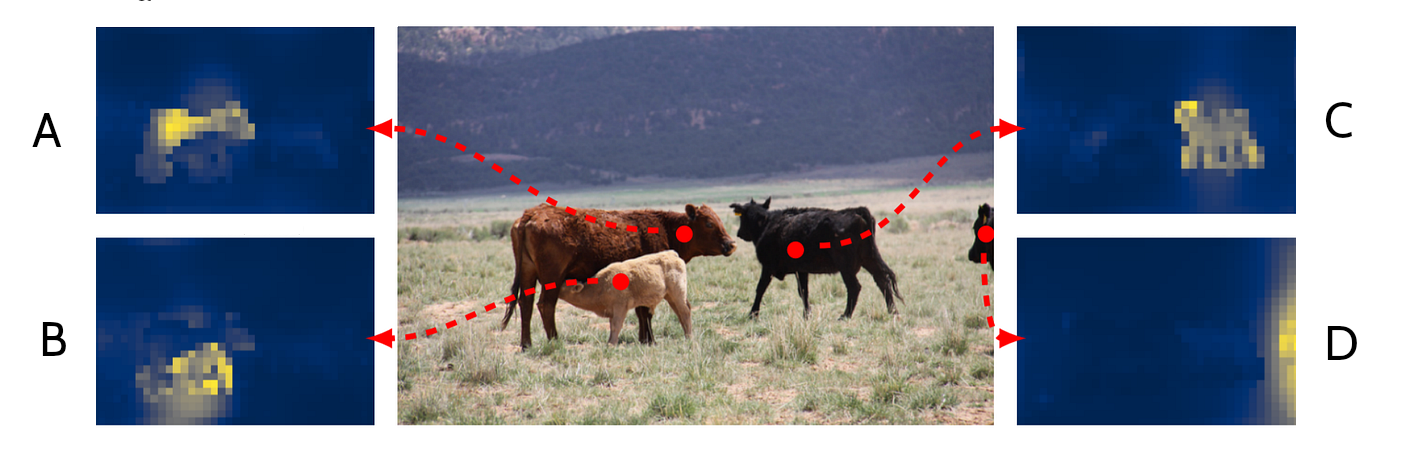
\includegraphics[width=0.8\textwidth]{Images/SOTA/attention.png}
    \caption{Encoder self-attention for a set of reference points. The encoder is able to separate individual instances (A-D). }
    \label{fig:attention}
\end{figure}

\subsection{Transformer}

Building on the attention mechanism, the transformer architecture was originally introduced for sequence modeling tasks in natural language processing, but has since proven highly versatile across domains. Its core innovation lies in replacing recurrent and convolutional operations with a stack of self-attention and feedforward layers, enabling efficient modeling of long-range dependencies.

A standard transformer consists of an encoder–decoder structure. For vision-related tasks such as image analysis and segmentation, typically only the encoder part is used, since the decoder was designed for sequence-to-sequence tasks like language translation. Each encoder layer is composed of two main components: a multi-head self-attention mechanism, which allows the model to jointly attend to information from different representation subspaces, and a position-wise feedforward network, which applies non-linear transformations independently to each position in the input.

To preserve information about the order or spatial position of elements, positional encodings are added to the input embeddings before they enter the encoder. Stacking multiple encoder layers enables the model to capture increasingly abstract and global relationships within the data. This ability to integrate long-range dependencies is particularly valuable in vision applications, including medical image analysis and cell segmentation, where spatial context plays a crucial role.

\begin{figure}[!ht]
    \centering
    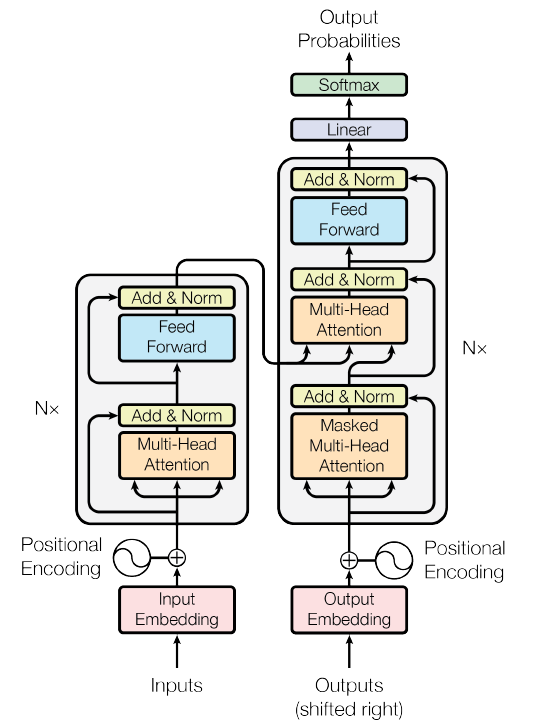
\includegraphics[width=0.5\textwidth]{Images/SOTA/transformer.png}
    \caption{Transformer architecture. For vision tasks, usually the left part (encoder) is taken.}
    \label{fig:transformer}
\end{figure}

\subsection{Vision Transformer}

The Vision Transformer (ViT) extends this transformer architecture from sequential data to image analysis by treating images as sequences of patches.
Instead of processing entire images using convolutional layers, ViT divides an image into fixed-size, non-overlapping patches, flattens them, and projects them into a lower-dimensional embedding space. These patch embeddings are then combined with positional encodings and fed into a standard transformer encoder.

ViTs have demonstrated strong performance in various computer vision tasks by leveraging the self-attention mechanism’s ability to model global dependencies between image regions, without the locality constraints of convolutional operations.

Although the vanilla ViT has shown impressive results on ImageNet, there are some theoretical concerns about the way vanilla ViT encode its features. 
While in CNN encoders, high- and low-res features are obtained in a corresponding layer depth, no such built-in multi-scale feature extraction is existent in vanilla ViTs. In addition, the non-overlapping, fixed-size tokenization of ViTs leads to high computational costs, as the complexity is $\mathcal{O}(N^2 \cdot D)$, scaling quadratically with the image size $N$ times the embedding dimension $D$.

\begin{figure}[!ht]
    \centering
    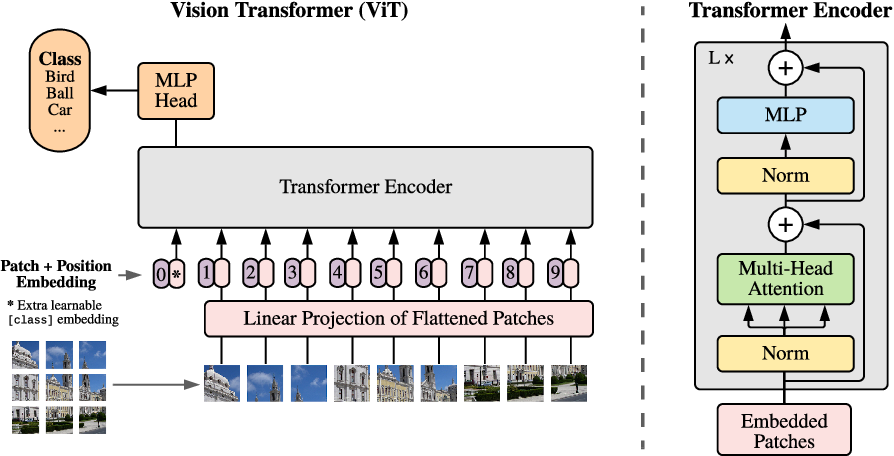
\includegraphics[width=0.9\textwidth]{Images/SOTA/vit.png}
    \caption{Vision transformer as presented in }
    \label{fig:vit}
\end{figure}


\subsection{SegFormer}

To tackle the above mentioned issues of the vanilla ViT, xy et al (cite) proposed the SegFormer architecture. It is composed of a hierarchical Transformer-based encoder and a lightweight decoder, designed specifically for efficient and accurate semantic segmentation. The encoder consists of multiple Mix Transformer (MiT) blocks, each incorporating three main components: efficient self-attention, Mix Feed-Forward Networks (Mix-FFN), and Overlapping Patch Mappings.

\begin{figure}[!ht]
    \centering
    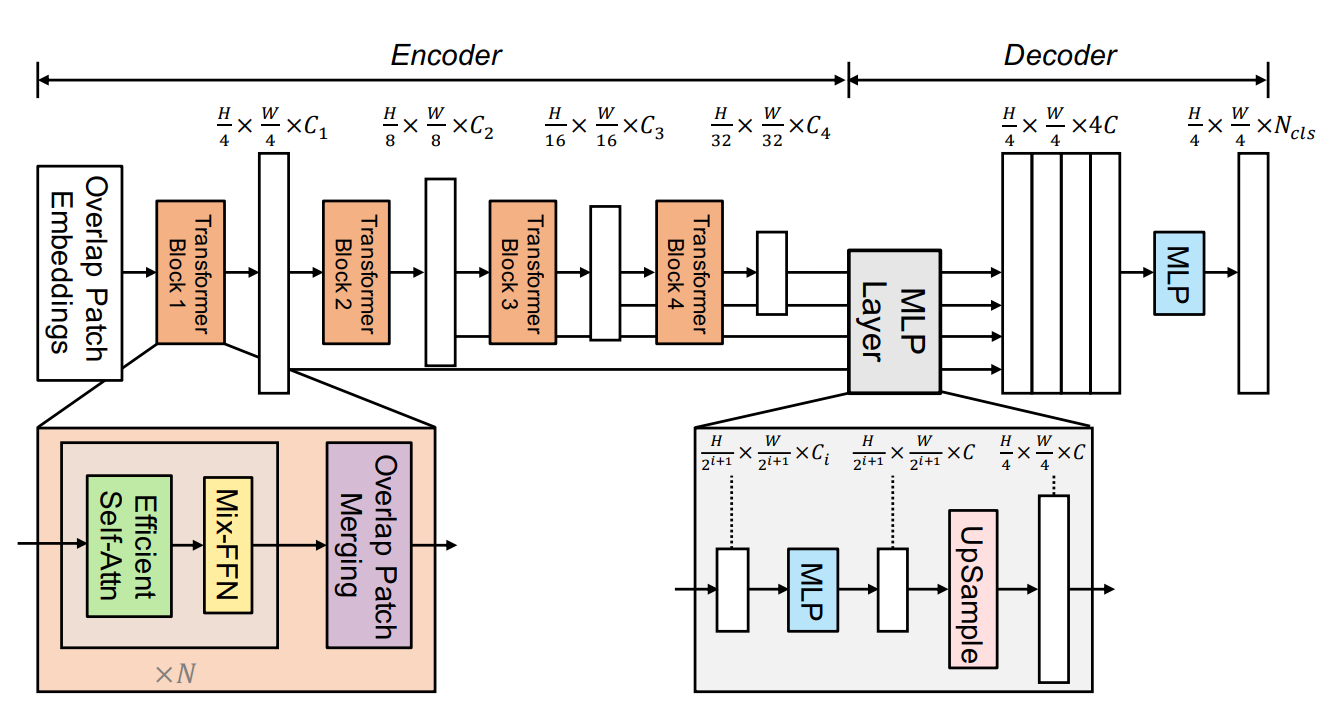
\includegraphics[width=0.9\textwidth]{Images/SOTA/SegFormer.png}
    \caption{SegFormer architecture as presented in}
    \label{fig:segformer}
\end{figure}

To reduce the computational complexity of the standard self-attention mechanism used in ViTs, they introduce an efficient self-attention variant: While the conventional self-attention has a complexity of $\mathcal{O}(pN^2)$, this is reduced to $\mathcal{O}(pN^2 / R)$ by modifying the key tensor $K$ as $K = \text{Linear}(\text{reshape}(K'))$, where $K' \in \mathbb{R}^{N/R \times C \cdot R}$, effectively grouping tokens into spatial regions. This significantly improves scalability on large input images. In the Mix-FFN, they replace positional encodings with a $3 \times 3$ depthwise convolution, which not only captures local spatial dependencies but also introduces an implicit positional bias, enabling the model to better encode structure. Overlapping Patch Mapping is used in each stage to partition the image into patches with shared pixels, preserving local continuity and reducing edge artifacts between patches. This patch merging is the main component of the downsampling part of the encoder. It thereby outputs multi-scale features from different stages, which are then processed by a lightweight decoder. The decoder projects all feature maps to a unified embedding space, upsamples them to a common resolution, and fuses them via concatenation. A linear prediction layer then generates per-pixel class logits. This minimalist decoder design ensures fast inference while maintaining segmentation accuracy. By combining hierarchical feature extraction, efficient attention, and a streamlined decoder, SegFormer achieves state-of-the-art performance across several benchmarks while remaining computationally lightweight. A diagram of the network architecture is depicted in figure \ref{fig:segformer}.

\subsection{MA-Net: Multi-Scale Attention Network}

The Multi-scale Attention Network (MA-Net), proposed by Fan et al., is a segmentation architecture designed to improve accuracy in medical image analysis, particularly for liver and tumor segmentation. It builds upon the encoder-decoder structure of U-Net, but enhances it with attention-based modules that enable the network to better capture long-range dependencies and multi-scale contextual information. MA-Net has been shown to outperform state-of-the-art models on the MICCAI 2017 LiTS Challenge. 

\begin{figure}[!ht]
    \centering
    \makebox[\textwidth]{%
    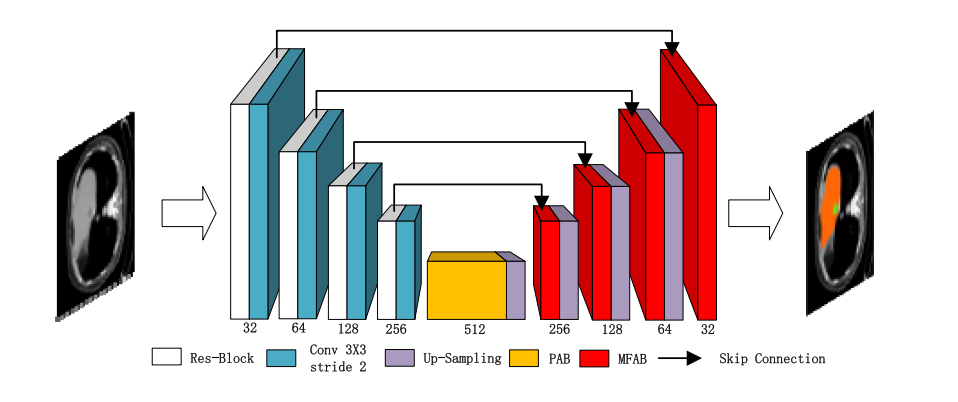
\includegraphics[width=1.0\textwidth]{Images/SOTA/MAnet.png}%
    }
    \caption{Architecture of the MA-Net. }
    \label{fig:MAnet}
\end{figure}


The encoder extracts hierarchical features through standard convolutional layers, while the attention-enhanced decoder refines these features using two sufisticated attention modules before producing the final segmentation output. Skip connections between encoder and decoder stages are preserved, allowing the network to retain important spatial information during upsampling. The full high level architecture is displayed in \ref{fig:MAnet}.


The key innovation in MA-Net lies in its decoder, which introduces two specialized attention modules: the \textit{Position-wise Attention Block} (PAB) and the \textit{Multi-scale Fusion Attention Block} (MFAB). 

The PAB is designed to model feature inter-dependencies in a global spatial context by computing position-aware attention maps, which helps the network focus on relevant regions within the entire image. 

\begin{figure}[!ht]
    \centering
    \makebox[\textwidth]{%
    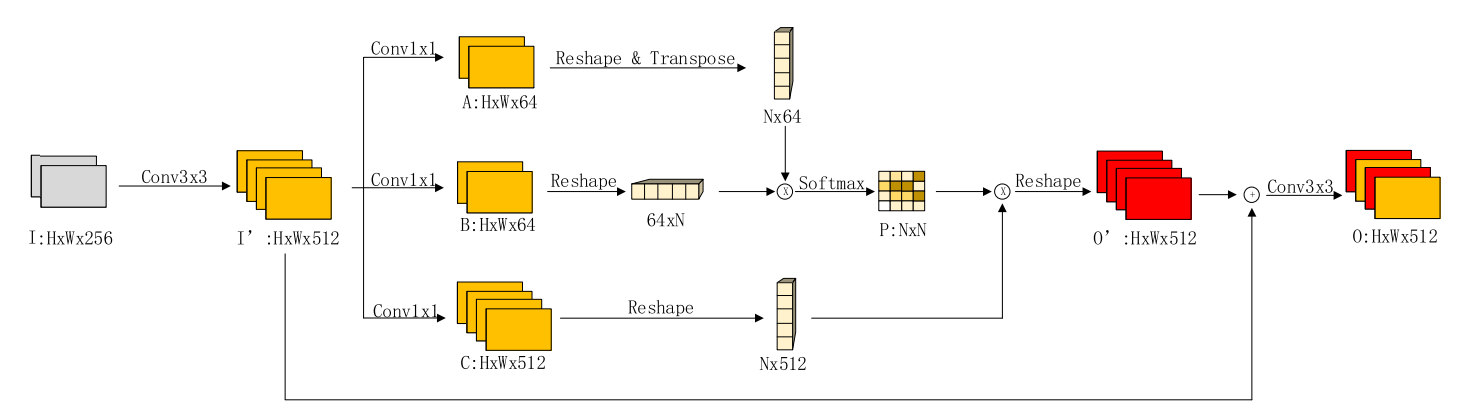
\includegraphics[width=1.2\textwidth]{Images/SOTA/PAB.png}%
    }
    \caption{Low-level view of the PAB block.}
    \label{fig:PAB}
\end{figure}

A low-level view of the PAB block is given in \ref{fig:PAB}. The local feature map $I \in \mathbb{R}^{H \times W \times 256}$ (in this net, the lowest resolution feature of the encoder) is first transformed by a $3 \times 3$ convolution to produce $I_0 \in \mathbb{R}^{H \times W \times 512}$. Three $1 \times 1$ convolution layers generate feature maps $A \in \mathbb{R}^{H \times W \times 64}$, $B \in \mathbb{R}^{H \times W \times 64}$, and $C \in \mathbb{R}^{H \times W \times 512}$. This basically mimics the learnable projection matrices (as defined in eq. \ref{Eq:2.1}) in transformers, turning input embeddings into pseudo $QKV$ representations. Reshaping $A$ and $B$ into $A \in \mathbb{R}^{N \times 64}$ and $B \in \mathbb{R}^{64 \times N}$, where $N = H \cdot W$ is the number of pixels, a matrix multiplication followed by softmax yields the spatial attention map $P \in \mathbb{R}^{N \times N}$:
\[
p_{ji} = \frac{\exp(A_i B_j)}{\sum_{i=1}^{N} \exp(A_i B_j)}.
\]
This map encodes the influence of the $i$-th position on the $j$-th position. The feature map $C$ (pseudo Key matrix) is reshaped to $C \in \mathbb{R}^{N \times 512}$, and multiplied with $P$ to obtain a context-aware representation:
\[
O'_j = \sum_{i=1}^{N} P_{ji} C_i.
\]
Finally, the result is reshaped back to $O'_0 \in \mathbb{R}^{H \times W \times 512}$, added element-wise to $I_0$, and passed through a $3 \times 3$ convolution to produce the final output $O \in \mathbb{R}^{H \times W \times 512}$:
\[
O_j = \alpha O'_j + I_{0,j},
\]
where $\alpha$ is a learnable scalar initially set to $0$. Each output position is thus a weighted sum of features across all positions combined with the original feature, providing a global contextual view that improves segmentation consistency. Note, that the matrix multiplication of $A$ and  $B$ is not normed as in the origin self-attention mechanism (see eq. \ref{Eq:2.2}). While this might reduce computational complexity, it makes the forward pass prone to overflow issues due to the lack of numerical stability from the norm operation.


The MFAB facilitates semantic feature fusion across multiple scales by combining feature maps of varying resolutions. This enables the decoder to integrate both fine-grained details and high-level semantic cues, which the authors claim to obtain more precise boundary delineation and region consistency. A low-level view of the MFAB block is given in \ref{fig:MFAB}.
\begin{figure}[!ht]
    \centering
    \makebox[\textwidth]{%
    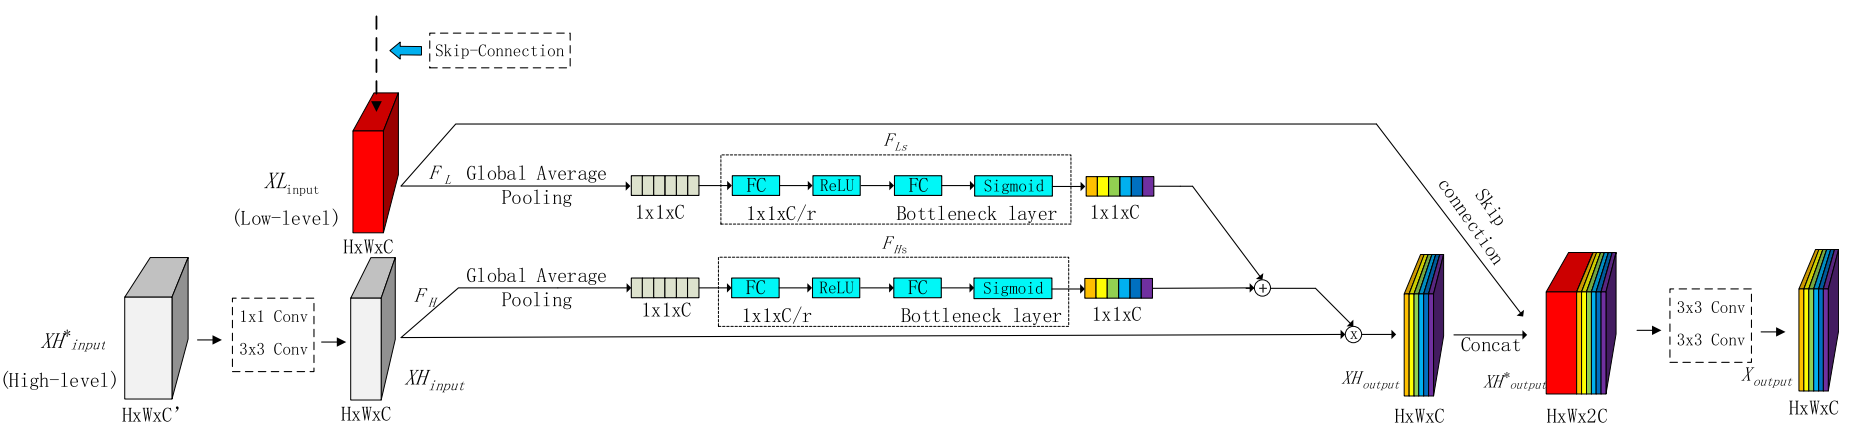
\includegraphics[width=1.2\textwidth]{Images/SOTA/MFAB.png}%
    }
    \caption{Multi-scale Fusion Attention Block (MFAB) structure. }
    \label{fig:MFAB}
\end{figure}


The high-level feature map $X_H^\ast \in \mathbb{R}^{H \times W \times C_0}$ is first transformed by a $3 \times 3$ convolution followed by a $1 \times 1$ convolution to obtain $X_H \in \mathbb{R}^{H \times W \times C}$, aligning it with the low-level skip feature $X_L \in \mathbb{R}^{H \times W \times C}$. Global average pooling is applied to both high- and low-level features to produce channel descriptors $s_c^{(H)}$ and $s_c^{(L)}$:
\[
s_c^{(H)} = \frac{1}{H W} \sum_{i=1}^{H} \sum_{j=1}^{W} X_H^{(c)}(i,j), \quad
s_c^{(L)} = \frac{1}{H W} \sum_{i=1}^{H} \sum_{j=1}^{W} X_L^{(c)}(i,j).
\]
These descriptors are passed through a bottleneck network with two fully connected layers (implemented as $1 \times 1$ convolutions in practice) with reduction ratio $r$ and activations ReLU ($\delta$) and sigmoid ($\sigma$) to obtain channel attention weights:
\[
z^{(H)} = \sigma \big( P_1 \, \delta(P_2 \, s^{(H)}) \big), \quad
z^{(L)} = \sigma \big( P_1 \, \delta(P_2 \, s^{(L)}) \big).
\]
The weights from high- and low-level features are combined by addition:
\[
z = z^{(H)} + z^{(L)},
\]
and the high-level feature map is rescaled channel-wise:
\[
\tilde{X}_H^{(c)} = z_c \cdot X_H^{(c)}.
\]
The rescaled high-level features are concatenated with the low-level skip features:
\[
X_{\text{concat}} = [\tilde{X}_H, X_L],
\]
and refined through two successive $3 \times 3$ convolutions to produce the final output:
\[
X_{\text{out}} = \text{conv2d}_{3 \times 3}(\text{conv2d}_{3 \times 3}(X_{\text{concat}})).
\]

Considering they basically reimplemented the concepts of Sequeeze and Exitement (SE) layers along with some concatinations and additions from two resolutions, the term attention may be a little misleading here. Nevertheless this way of scaling feature maps with fused SE results has been proven to perform really well.


\section{Masked Autoencoders}

Masked Autoencoders (MAE) are a self-supervised learning framework designed to pretrain large vision models efficiently. The key idea is to randomly mask a high proportion of image patches and to train the network to reconstruct the missing pixels from the remaining visible content. This forces the model to learn meaningful representations of visual structures, as it must capture global context in order to accurately fill in the missing regions. 

\begin{figure}[!ht]
    \centering
    \makebox[\textwidth]{%
    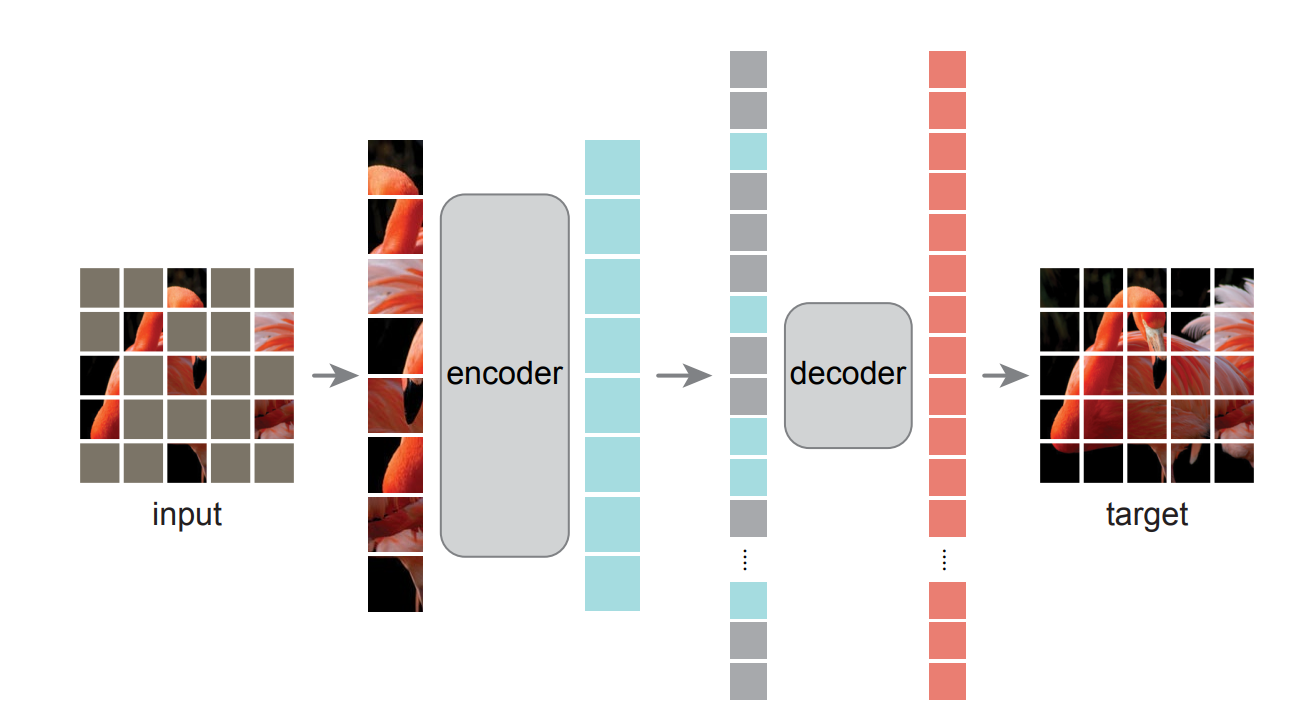
\includegraphics[width=1.0\textwidth]{Images/SOTA/MAE.png}%
    }
    \caption{MAE architecture as presented in \cite{LeCun.1989}.}
    \label{fig:MAE}
\end{figure}

The architecture of an MAE is based on an asymmetric encoder–decoder design. The encoder processes only the subset of visible patches without introducing explicit mask tokens. This makes the encoder highly efficient, as it avoids computation over large portions of the input image. The decoder, by contrast, is lightweight and is responsible for reconstructing the original image from the latent representation of the visible patches in combination with the mask tokens that indicate the missing regions. In this way, most of the modeling capacity is allocated to the encoder, while the decoder only serves as a reconstruction head during pretraining. 

This design enables masked autoencoders to train large models efficiently and effectively. Compared to traditional supervised pretraining approaches, MAEs achieve significant gains in training speed, with reported improvements of up to a threefold acceleration, while also improving downstream accuracy. After pretraining, the decoder is discarded, and the encoder is applied to complete, unmasked images. The pretrained encoder then serves as a powerful feature extractor for a variety of recognition and segmentation tasks, often providing strong performance with limited additional task-specific training. 



\section{Segment Anything}

The Segment Anything Model (SAM) represents a new class of foundation models for image segmentation. Unlike conventional approaches that are trained for a specific downstream task, SAM is designed as a promptable segmentation model: given an image and a prompt, it returns a valid segmentation mask. Prompts specify what to segment and can be provided in different forms, including spatial inputs such as points, bounding boxes or scribbles, or textual descriptions such as “a cat with black ears.” A central requirement is that the model always outputs a reasonable mask, even in cases of ambiguity, by producing at least one plausible segmentation result. 

The training objective of SAM is a promptable segmentation task, which allows the model to generalize across a wide range of domains. Downstream applications can be reformulated as prompt engineering, which makes it possible to reuse the same foundation model for diverse segmentation problems without additional training. The design of SAM therefore emphasizes three objectives: the ability to support heterogeneous prompts, the ability to deliver results quickly enough for interactive use, and explicit handling of ambiguous prompts. 

\begin{figure}[!ht]
    \centering
    \makebox[\textwidth]{%
    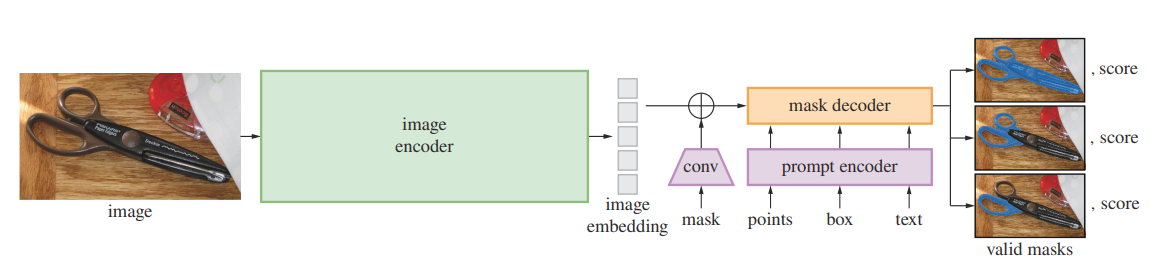
\includegraphics[width=1.0\textwidth]{Images/SOTA/SAM1.png}%
    }
    \caption{MAE architecture as presented in \cite{LeCun.1989}.}
    \label{fig:SAM1}
\end{figure}

The architecture of SAM is composed of three decoupled components: an image encoder, a prompt encoder, and a mask decoder. The image encoder is actually just a vanilla ViT with small adaptations, such as the choice of global attention computation on only a few layers and different embedding dimensions for specific size versions (small, medium, large, huge), each pretrained in a masked autoencoder style. The image encoder processes an input image once to compute a dense embedding, which can then be reused for multiple prompts. This amortization of computational cost is crucial for interactive applications. The prompt encoder embeds different forms of prompts, whether spatial or textual, into a common representation. The mask decoder then fuses image and prompt embeddings to predict segmentation masks. It employs a modified Transformer decoder block with both self-attention over prompts and bidirectional cross-attention between prompt and image embeddings. After two decoding blocks, the image embedding is upsampled and an MLP maps the output tokens to a dynamic linear classifier, which produces per-pixel mask probabilities. 

To handle ambiguity, the decoder generates multiple candidate masks for a single prompt. During training, only the mask with the lowest loss, corresponding to the best overlap with the ground truth, is used for backpropagation. An additional branch predicts the intersection-over-union score for each mask, which enables the ranking of the different outputs at inference time. The loss functions used in training combine focal loss and Dice loss with a strong weighting toward focal loss, while the IoU prediction branch is supervised with mean squared error. 

A key factor in SAM’s ability to generalize is the unprecedented scale of its training data. To create such a dataset, the authors developed a data engine, a model-in-the-loop annotation strategy with three progressive stages. In the assisted-manual stage, SAM supported human annotators in producing masks, similar to classical interactive segmentation. In the semi-automatic stage, the model was able to generate masks for a subset of objects automatically, while annotators concentrated on refining difficult cases. Finally, in the fully automatic stage, SAM was prompted with a grid of points, producing on average around 100 high-quality masks per image. This pipeline resulted in the SA-1B dataset, which contains more than one billion masks from eleven million licensed and privacy-preserving images. Compared to existing segmentation datasets, this is larger by two orders of magnitude and provides the foundation for SAM’s strong generalization abilities. 


\subsection{Segment Anything 2}

Following the release of the original Segment Anything Model, a second version (SAM 2) was introduced to further improve versatility and applicability. While SAM 1 demonstrated the feasibility of promptable segmentation at scale, SAM 2 extends these capabilities with a stronger focus on efficiency, scalability, and temporal reasoning. 

SAM 2 preserves the core idea of promptable segmentation with a decoupled architecture of image encoder, prompt encoder, and mask decoder, but introduces several refinements. The image encoder is optimized for faster inference, making the model more practical for large-scale or interactive applications. Moreover, SAM 2 improves ambiguity handling by refining the multi-mask output strategy, leading to more consistent predictions in complex scenes. 

A key extension of SAM 2 lies in its support for \textit{video and spatio-temporal segmentation}. By incorporating mechanisms to reuse information across frames, SAM 2 enables object tracking and segmentation over time, which broadens its applicability beyond static image analysis. At the same time, the training data has been further scaled, with an expanded dataset that improves robustness across domains and object categories. 


\subsection{Hiera}
Hiera is a hierarchical vision transformer architecture designed to combine the strengths of transformer-based models with the efficiency of convolutional networks. Unlike standard Vision Transformers, which operate on a flat sequence of image patches, Hiera introduces a hierarchical structure that progressively reduces spatial resolution while expanding the feature dimension. This design mirrors the multiscale feature extraction used in convolutional neural networks and is particularly well-suited for dense prediction tasks such as segmentation. 

\begin{figure}[!ht]
    \centering
    \makebox[\textwidth]{%
    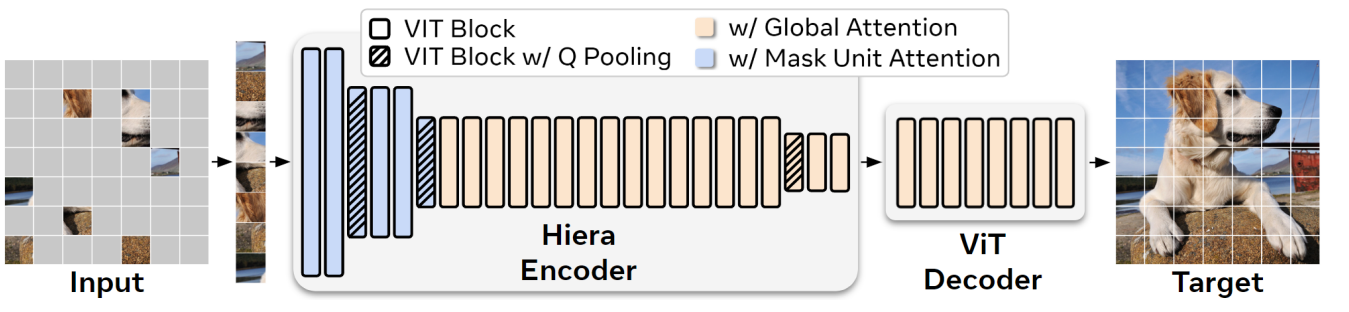
\includegraphics[width=1.0\textwidth]{Images/SOTA/Hiera.png}%
    }
    \caption{MAE architecture as presented in \cite{LeCun.1989}.}
    \label{fig:Hiera}
\end{figure}

The model is constructed as a stack of transformer blocks organized into stages. Each stage processes tokens at a given spatial resolution before applying patch merging to reduce resolution and increase the channel dimension. This hierarchical representation enables the network to capture both fine-grained local patterns and coarse global context. In addition, Hiera incorporates efficient attention mechanisms that scale sub-quadratically with image size, making it computationally more efficient than standard ViT backbones while retaining strong modeling capacity. 

A key advantage of Hiera is its flexibility as a general-purpose backbone. It can be pretrained on large-scale image classification tasks and subsequently fine-tuned for a wide range of downstream applications, including semantic segmentation, instance segmentation, and object detection. Empirical studies have shown that Hiera achieves competitive accuracy compared to state-of-the-art transformer backbones, while offering improved efficiency and scalability across different model sizes. 

\section{Mediar}

Mediar is yet another encoder decoder style architecture, designed specifically for cell segmentation. It was developed in the context of the 2022 NeurIPS Cell Segmentation Challenge, where it achieved top performance across a variety of imaging modalities. Their approach is based on the Cellpose learning objective, but instead of using a U-Net style CNN backbone, they adopt the encoder part of SegFormer and combine it with the decoder blocks of MA-Net. This still ensures a hierarchical feature integration from the SegFormer multi-resolution features, to the MFAB blocks of the MA-Net via skip connections. They use Mish in the encoder and decoder for better generalization.  Although prior work use a single segmentation head, meaning they map the features to a single output tensor with multiple channels for each output (cell probability, x- and y- flows), the authors used two seperate heads to map features to the cell probability and flows, respectively. They argue that semantic prediction for the objects and mse regression for the spatial gradient field interfers with each other, while using the same feature space \cite{caruana}. Therefore, they use two seperate conv2d layers with batch norm to map the features to the respective outputs.

\begin{figure}[!ht]
    \centering
    \makebox[\textwidth]{%
    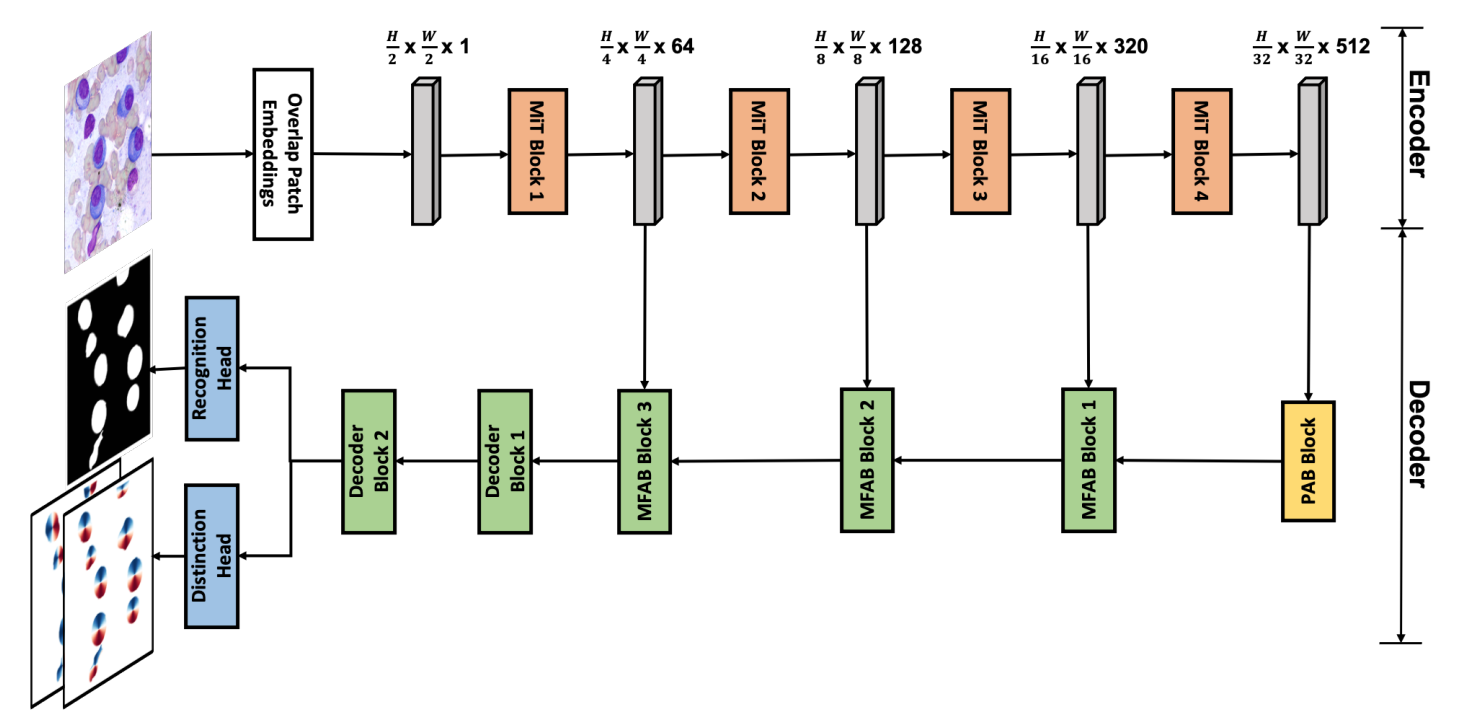
\includegraphics[width=1.0\textwidth]{Images/SOTA/mediar_net.png}%
    }
    \caption{Encoder embeddings of the train set clustered with k-mean and intuition of amlplified sampling \cite{LeCun.1989}.}
    \label{fig:mediar_net}
\end{figure}


They pretrained MEDIAR on a large set of public datasets, namely Omnipose, Cellpose, Livecell and DataScienceBowl-2018, which makes a combined total of 7,242 labeled images. For the Challenge Dataset, they came up with a sophisticated way of training two seperate models (phases) with each different subsets of challenge data in the pretraining set, to perform ensembling prediction at test time. In the first phase, the net is initialized with ImageNet-1k pretrained encoder weights, and further trained on the public datasets for 80 epochs to establish strong general-purpose cell representations. In the second phase, this model was further trained for 60 epochs on the combined set of public datasets and the challenge training data, allowing the network to bridge between general cell morphologies and the specific modalities of the target domain. Fine-tuning was then conducted separately on the models from both phases. The phase 1 model was fine-tuned for 200 epochs on the challenge training set, specializing it to modalities present only in the target data. The phase 2 model was fine-tuned for 25 epochs, leveraging its broader knowledge of both public and challenge domains. Interestingly, the two models exhibited complementary behavior: the phase 1 fine-tuned model excelled at adapting to unseen modalities in the challenge, whereas the phase 2 fine-tuned model maintained stronger generalization across shared modalities. To further enhance robustness, they introduced a relabeling step at phase 2 fine-tuning, correcting images where the pretrained and phase 1 fine-tuned models produced misaligned predictions, thereby mitigating the impact of noisy annotations.
Similarly to the style embeddings from Cellpose, they examine modality dependent embeddings in the pretraining dataset. To do that, they cluster the encoder embeddings from the phase-1 pretrained model using k-means with 40 clusters. They observed an uneven distribution across samples and concluded it might negatively impact model performance on underrepresented modalities. To mitigate this, they balance the sampling ratio in training by over-sampling underrepresented clusters, ensuring that the model receives a more uniform exposure to all modalities. Figure \ref{fig:latent_modalities} illustrates the discovered latent modalities and the corresponding sample amplification strategy.

\begin{figure}[!ht]
    \centering
    \makebox[\textwidth]{%
    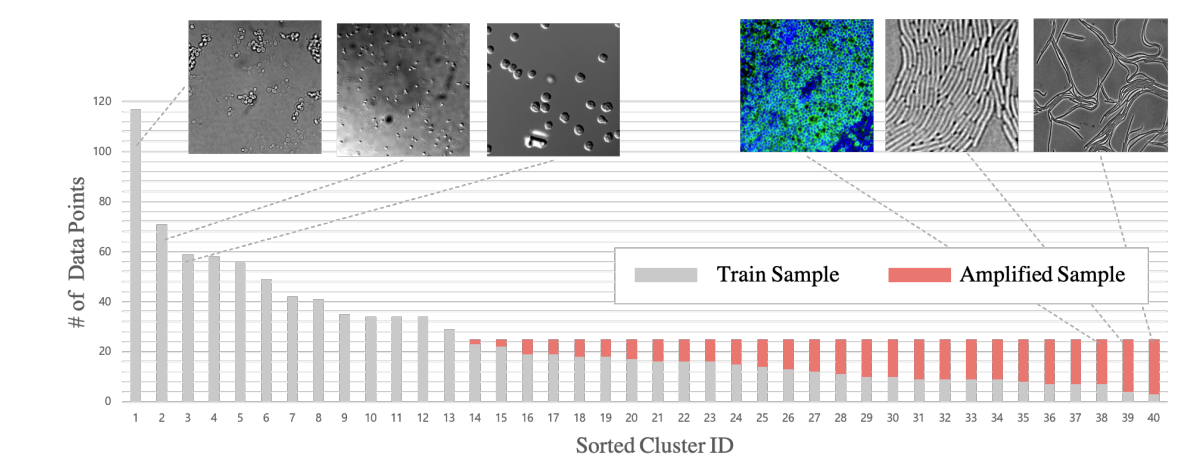
\includegraphics[width=1.0\textwidth]{Images/SOTA/latent_modalities.png}%
    }
    \caption{Encoder embeddings of the train set clustered with k-mean and intuition of amlplified sampling \cite{LeCun.1989}.}
    \label{fig:latent_modalities}
\end{figure}

This transformer-based backbone performed really well in the challenge, but the authors of Cellpose were sceptical about the benchmarkings, claiming that conditions for pretraining of the Cellpose model were impaired. This sparked a debate about the feasibility of transformer-based models being superior to CNN backbones in the cell segmentation domain. From a theoretical perspective, this is not very simple. While the inductive bias of CNNs makes them limited to a certain receptive field but also very data efficient, transformers are able to capture long-range dependencies and global context, which may or may not be beneficial, depending on the specific task and dataset.


\section{CellposeSAM}

CellposeSAM is a very recent extention of the original Cellpose model. Since the initial launch of Cellpose1, the field of computer vision has seen significant advancements, particularly with the introduction of foundation models like the Segment Anything Model (SAM). These models have demonstrated remarkable capabilities in generalizing across diverse image domains. Motivated by these developments, the authors of CellposeSAM decided to integrate the strengths of SAM into the Cellpose framework to enhance its segmentation performance and versatility. Interestingly, they did not use the original SAM decoder, but rather combined the image encoder of SAM1 with the Cellpose learning objective. So from a high-level perspective, CellposeSAM is just Cellpose1 with a ViT, instead of the CNN backbone. For the ViT, there are only minor adjustments such as reduced patch size from 16x16 to 8x8 and input spatial dimensions from 1024x1024 to 256x256. For the local attention layers in the original SAM1, they changed all layers to global attention instead of only global in layers 6, 12, 18 and 24. In contrast to Mediar and Cellpose1, they do not use hierarchical features from different stages of the encoder, but only the output of the last encoder layer. So decoder of the network is composed of just one conv2d layer, which converts the ViT encoder neck to the cellpose learning objective. An additional, deterministic fixed kernel transposeConv2d layer is used to transform the image from token to pixel space. The resulting model with an order of magnitude more parameters (305M vs 44M) compared to the original Cellpose1, which makes it impractical to run without a GPU. 

\begin{figure}[!ht]
    \centering
    \makebox[\textwidth]{%
    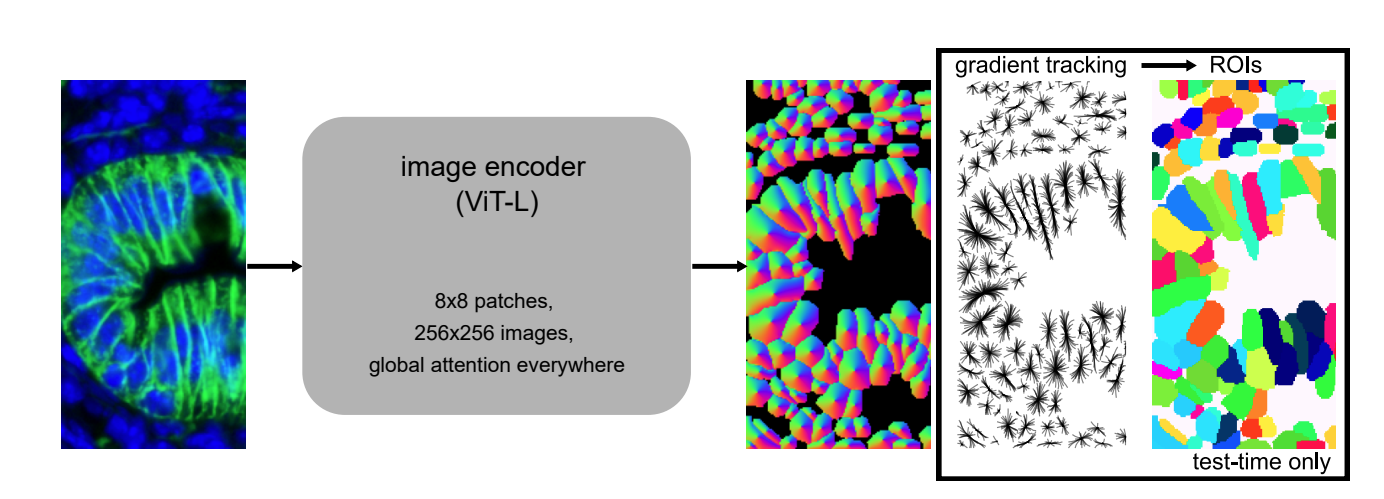
\includegraphics[width=1.0\textwidth]{Images/SOTA/cellposeSam.png}%
    }
    \caption{Encoder embeddings of the train set clustered with k-mean and intuition of amlplified sampling \cite{LeCun.1989}.}
    \label{fig:cellposesam}
\end{figure}

A major strength of CellposeSAM is the broad range of pretraining data. Weights are initialized with the SAM weights pretrained on the SA-1B dataset \ref{Kirillov}, and further trained on an updated dataset of cells and nuclei containing 22,826 train images with a combined 3,341,254 training regions of interest (ROIs). This leads to a really good performance on various types of cell- and imaging modalities, as they outperform or match other models on all datasets they tested on, setting a new state-of-the-art on cellular segmentation benchmarks.

